% enable this to activate the version for PRINT
% disable this to make the pdf symmetric and without white pages
% => asymmetric alternating left/right margins
% \newcommand*{\printversion}{}%

%% | ---------------- document meta information --------------- |

\newcommand{\Author}{John Smith}
\newcommand{\Department}{Department of Cybernetics}
\newcommand{\Supervisor}{Ing. My Supervisor, Ph.D.}
\newcommand{\SupervisorSpecialist}{Ing. My Specialist, Ph.D.}
\newcommand{\Programme}{Electrical Engineering and Information Technology}
\newcommand{\Field}{Artificial Intelligence and Biocybernetics}
\newcommand{\Title}{My Thesis Title\\[0.5em]Can Span Multiple Lines}
\newcommand{\Keywords}{Unmanned Aerial Vehicles, Automatic Control}
\newcommand{\KlicovaSlova}{Bezpilotní Prostředky, Automatické Řízení}
\newcommand{\Year}{2021}
\newcommand{\Month}{January}
\newcommand{\Date}{\Month~\Year}
\newcommand{\Location}{Prague}

%% | ---------------------- configuration --------------------- |

% most of the configuration stuff happens here
%!TEX root = ../main.tex

%% | ----------------------- page setup ----------------------- |

% define documentclass based on the print/screen version of the document
\pdfoutput=1
\ifdefined\printversion
  \documentclass[a4paper,11pt,twoside,openright]{book}
\else
  \documentclass[a4paper,11pt,oneside]{book}
\fi

% define how "clearpage" works with the print/screen version of the document
\newcommand{\conditionalClearPage}{
  \ifdefined\printversion
    \cleardoublepage
  \else
    \clearpage
  \fi
}

%% | ----------------- commonly used packages ----------------- |

\usepackage[english]{babel}
\usepackage[utf8]{inputenc}
\usepackage{csquotes}
\usepackage{amsmath,amsfonts,amssymb,bm}
\usepackage{nicefrac}
\usepackage{algorithm,algpseudocode}
\usepackage[title,titletoc]{appendix}
\usepackage{latexsym}
\usepackage{a4wide}
\usepackage{color}
\usepackage{indentfirst}
\usepackage{graphicx}
\usepackage{fancyhdr,lastpage}
\usepackage{longtable}
\usepackage{pifont}
\usepackage{makeidx}
\usepackage{multirow}
\usepackage{dcolumn}
\usepackage{epstopdf}
\usepackage{xurl}
\usepackage{listings}
\usepackage{relsize}
\usepackage{pdfpages}
%\usepackage{url}
\usepackage{lipsum}
\usepackage{isotope}
\usepackage{verbatim}
\usepackage{xcolor}
\usepackage{tcolorbox}
\usepackage[hidelinks]{hyperref}
\usepackage{multicol}
\usepackage{subfig}
\usepackage[export]{adjustbox}
\usepackage{amsmath} 
\usepackage{alertmessage}
\usepackage{hyperref}
% print version has different margins to accommodate the spine of the book
% do not move this around, or it stops working
\ifdefined\printversion
  \usepackage[a4paper,margin=3.2cm,inner=3.4cm,outer=2.0cm]{geometry}
\else
  \usepackage[a4paper,margin=3.2cm,inner=2.7cm,outer=2.7cm]{geometry}
\fi

\hyphenation{}

%% | ---------------------- abbreviations --------------------- |

\usepackage[printonlyused]{acronym}

% use to change margins around abbreviations block
\def\changemargin#1#2{\list{}{\rightmargin#2\leftmargin#1}\item[]}
\let\endchangemargin=\endlist

%% | -------------------------- tikz -------------------------- |

\usepackage{tikz}
\usepackage{pgfplots}
\pgfplotsset{compat=1.14}
\usetikzlibrary{backgrounds,arrows,automata,shapes,positioning,calc,through,spy,shapes,shapes.geometric,shapes.multipart,fit,patterns,fadings}
\pgfdeclarelayer{background}
\pgfdeclarelayer{foreground}
\pgfsetlayers{background,main,foreground}

%% | ------------ siunitx for units of measurements ----------- |

\usepackage{siunitx}
\DeclareSIUnit \parsec {pc}
\DeclareSIUnit \electronvolt {eV}
\DeclareSIUnit \pixel {px}
\DeclareSIUnit \arcmin {arcmin}
\DeclareSIUnit \erg {erg}
\DeclareSIUnit \joul {J}

%% | --------------- change formatting of lists --------------- |

\usepackage{enumitem}
\setlist{nosep}

%% | -------------------- table of contents ------------------- |

\usepackage[subfigure]{tocloft}

\tocloftpagestyle{plain}

%% | ----------------- formatting of a chapter ---------------- |

\usepackage{titlesec}
\titleformat{\chapter}[block]
{\normalfont\huge\bfseries}{Chapter \thechapter\\\vspace{0.1em}\\}{1em}{\Huge}
% {?}{before}{after}
\titlespacing*{\chapter}{0pt}{-1em}{2em}

%% | ------------------------ biblatex ------------------------ |

\usepackage[backend=bibtex,defernumbers=true,style=ieee,sorting=ydnt,sortcites=true]{biblatex}

% define the source file with bibliography
\addbibresource{main.bib}

\renewcommand*{\bibfont}{\Font}

% add suffix "a" to publications containing the keyword "mine"
% add suffix "c" to publications containing the keyword "mine" && "core"
\DeclareFieldFormat{labelnumber}{%
  \ifkeyword{mine}
    {\ifkeyword{core}
      {{\number\numexpr#1}c}%
      {{\number\numexpr#1}a}%
    }%
    {#1}%
}

\DeclareCiteCommand{\tabcite}%[\mkbibbrackets]
  {\usebibmacro{cite:init}%
   \usebibmacro{prenote}}
  {\usebibmacro{citeindex}%
   \usebibmacro{cite:comp}}
  {}
  {\usebibmacro{cite:dump}%
   \usebibmacro{postnote}}

% define fullciteinbox command
\definecolor{light-gray}{gray}{0.95}
\newcommand{\fullciteinbox}[2]{%

\DeclareCiteCommand{\fullcite}
{\usebibmacro{prenote}}
{\clearfield{addendum}%
  \usedriver
  {\defcounter{minnames}{6}%
  \defcounter{maxnames}{6}}
{\thefield{entrytype}}}
{\multicitedelim}
{\usebibmacro{postnote}}

\begin{tcolorbox}[width=\textwidth,colback={light-gray},title={}]%
\ifx&#2&
\else
  \textbf{#2}:\\\\
\fi
\begin{minipage}[t]{0.07\linewidth}%
\raggedright%
\cite{#1}%
\end{minipage}%
\begin{minipage}[t]{0.93\linewidth}%
\fullcite{#1}%
\end{minipage}%
\end{tcolorbox}%
%}%
\vspace{-0.3em}
}%

% change the bibliography font style
% does not compile without this
\let\bibfont\small

%% | ---------------------- custom macros --------------------- |

\newcommand{\strong}[1]{\textbf{#1}}
\newcommand{\coord}[1]{\textbf{#1}}
\newcommand{\norm}[1]{\left\lvert#1\right\rvert}
\newcommand{\m}[1]{\ensuremath{\mathbf{#1}}}
\newcommand\numberthis{\addtocounter{equation}{1}\tag{\theequation}}
\newcommand{\add}[1]{{\color{green} {#1}}}
\newcommand{\todo}[1]{{\color{red} TODO {#1}}}
\newcommand{\updated}[1]{{\color{blue} {#1}}}
\newcommand{\real}{\mathbb{R}}
\newcommand{\red}[1]{{\color{red} #1}}
\newcommand{\minus}{\scalebox{0.75}[1.0]{$-$}}
\newcommand{\plus}{\scalebox{0.8}[0.8]{$+$}}
\newcommand{\figvspace}{\vspace{-1em}}

% referencing
\newcommand{\reffig}[1]{Fig.~\ref{#1}}
\newcommand{\reflst}[1]{Lst.~\ref{#1}}
\newcommand{\refalg}[1]{Alg.~\ref{#1}}
\newcommand{\refsec}[1]{Sec.~\ref{#1}}
\newcommand{\reftab}[1]{Table~\ref{#1}}
\newcommand{\refeq}[1]{\eqref{#1}}

%% | ----------------- listings - showing code ---------------- |

\usepackage{listings}     
\usepackage{lstautogobble}  % Fix relative indenting
\usepackage{color}          % Code coloring
\usepackage{zi4}            % Nice font

\definecolor{bluekeywords}{rgb}{0.13, 0.13, 1}
\definecolor{greencomments}{rgb}{0, 0.5, 0}
\definecolor{redstrings}{rgb}{0.9, 0, 0}
\definecolor{graynumbers}{rgb}{0.5, 0.5, 0.5}

\usepackage{listings}
\lstset{
    autogobble,
    columns=fullflexible,
    showspaces=false,
    showtabs=false,
    breaklines=true,
    showstringspaces=false,
    breakatwhitespace=true,
    escapeinside={(*@}{@*)},
    commentstyle=\color{greencomments},
    keywordstyle=\color{bluekeywords},
    stringstyle=\color{redstrings},
    numberstyle=\color{graynumbers},
    basicstyle=\ttfamily\footnotesize,
    frame=l,
    framesep=12pt,
    xleftmargin=12pt,
    tabsize=4,
    captionpos=b
}

%% | -------------------- layout parameters ------------------- |

% no indent, free space between paragraphs
\setlength{\parindent}{1cm}
\setlength{\parskip}{1ex plus 0.5ex minus 0.2ex}

% offsets the head down
\setlength{\headheight}{18pt}

% foot line
\renewcommand{\footrulewidth}{0.4pt}

%% | -------------- define the 'full' page style -------------- |

\fancypagestyle{full}{%

  % clear the default layout
  \fancyhead{}
  \fancyfoot{}

  % page header
  \fancyhead[LO]{\leftmark}
  \fancyhead[RE]{\rightmark}
  \fancyhead[LE,RO]{\thepage/\pageref{LastPage}}

  % page footer
  \fancyfoot[L]{CTU in Prague}
  \fancyfoot[R]{\Department}
  \fancyfoot[C]{}
}

%% | -------------- define the 'plain' page style ------------- |

\fancypagestyle{plain}{%

  % clear the default layout
  \fancyhead{}
  \fancyfoot{}

  % page header
  \fancyhead[LE,RO]{\thepage}
}

%% | -------------- Adjust style of chapter names ------------- |

\renewcommand{\chaptermark}[1]{\markboth{\MakeUppercase{\thechapter.\ #1}}{}}

%% | -------- European layout, no extra space after '.' ------- |

\frenchspacing

%% | ----------- adjust the style of the first page ----------- |

\makeatletter
\renewcommand\chapter{\if@openright\cleardoublepage\else\clearpage\fi
                    \thispagestyle{full}% original style: plain
                    \global\@topnum\z@
                    \@afterindentfalse
                    \secdef\@chapter\@schapter}
\makeatother


%% | ---------------------- the contents ---------------------- |

\begin{document}

\pagenumbering{roman}

%% --------------------------------------------------------------
%% |                         Title page                         |
%% --------------------------------------------------------------

%!TEX root = ../main.tex

\begin{titlepage}
  \begin{center}

    \textsc{\Large Czech Technical University in Prague}\\[1em]
    \textsc{\large Faculty of Electrical Engineering\\
    \Department\\
    Multi-robot Systems\\[3em]
    }
    
\includegraphics[height=4.1cm]{fig/ctu_lion.pdf}\\[3em]

    \textbf{\textsc{\Huge \Title}}\\[2em]

    \textbf{\Large Bachelor's Thesis}\\[6em]

    \textbf{\huge \Author}\\[6em]

    {\large \Location, \Date}\\[3em]

    Study programme: \Programme\\
    Branch of study: \Field\\[4em]

    \textbf{Supervisor: \Supervisor}\\

    \vspace{2pt}

  \end{center}
\end{titlepage}


% set up the page style for the "intro" pages
\pagestyle{plain}

%% --------------------------------------------------------------
%% |                       Acknowledgments                      |
%% --------------------------------------------------------------

\conditionalClearPage

%!TEX root = ../main.tex

\section*{Acknowledgments}
%First of all, I would like to express my gratitude to my supervisor for all his support, guidance and valuable advices during this project.
%Secondly, I want to express my appreciation to my classmates and colleagues for the all the well spend study time, many and many created memes and mutual support during our challenging study period.
%I am also thankful to my family for all the support they provided my during my studies. %, that  forget to thank my family for all their support throughout my studies.
%Finally, I would like to express my appreciation to everyone who ensures that the research topic of this work would never be needed in practice, and that the radiation situation in Czechia, in Ukraine and everywhere else) would "remain normal."
First of all, I would like to express my gratitude to my supervisor for all his support, guidance, and valuable advice during this project.
Secondly, I want to express my appreciation to my classmates and colleagues for the time we spent studying together, the countless memes we created, and the mutual support we provided each other during our challenging study period.
I am also thankful to my family for their unwavering support throughout my studies.
Finally, I would like to express my appreciation to everyone who ensures that the research topic of this work would never be needed in practice and that the radiation situation in Czechia, Ukraine, and everywhere else in the world remains normal.

\vspace{2.5cm}








\section*{Poděkování}
Nejprve bych rád vyjádřil svou vděčnost svému vedoucímu za veškerou podporu, vedení a cenné rady během tohoto projektu. 
Zadruhé bych chtěl vyjádřit své díky svým spolužákům a kolegům za čas, který jsme spolu strávili studiem, nespočet vytvořených memů a vzájemnou podporu během našeho náročného studijního období. 
Jsem také vděčný své rodině za jejich neochvějnou podporu během celého mých studií. 
Nakonec bych chtěl vyjádřit své uznání všem, kdo se starají o to, aby výzkumné téma této práce nebylo nikdy potřeba v praxi a aby radiační situace v České republice, na Ukrajině a všude jinde zůstala normální.

%Chtwl bych poděkovat vedoucímu mé práce za veškerou podporu, cenné rady a předané zkušenosti.
%Zadruhé děkuji svým spolužákům a kolegů za všechen ten čas společně strávený studiem, mnoho a mnoho vytvořených memů a vzájemnou podporu během náročných studií.
%Děkuji také své rodině za veškerou podporu během celé doby studia.
%Nakonec bych chtěl poděkovat všem, kteří se starají o to, aby výzkumné téma této práce nebylo nikdy potřeba v praxi a radiační situace zůstávala normální. 


%% --------------------------------------------------------------
%% |                         Assignment                         |
%% --------------------------------------------------------------

\conditionalClearPage

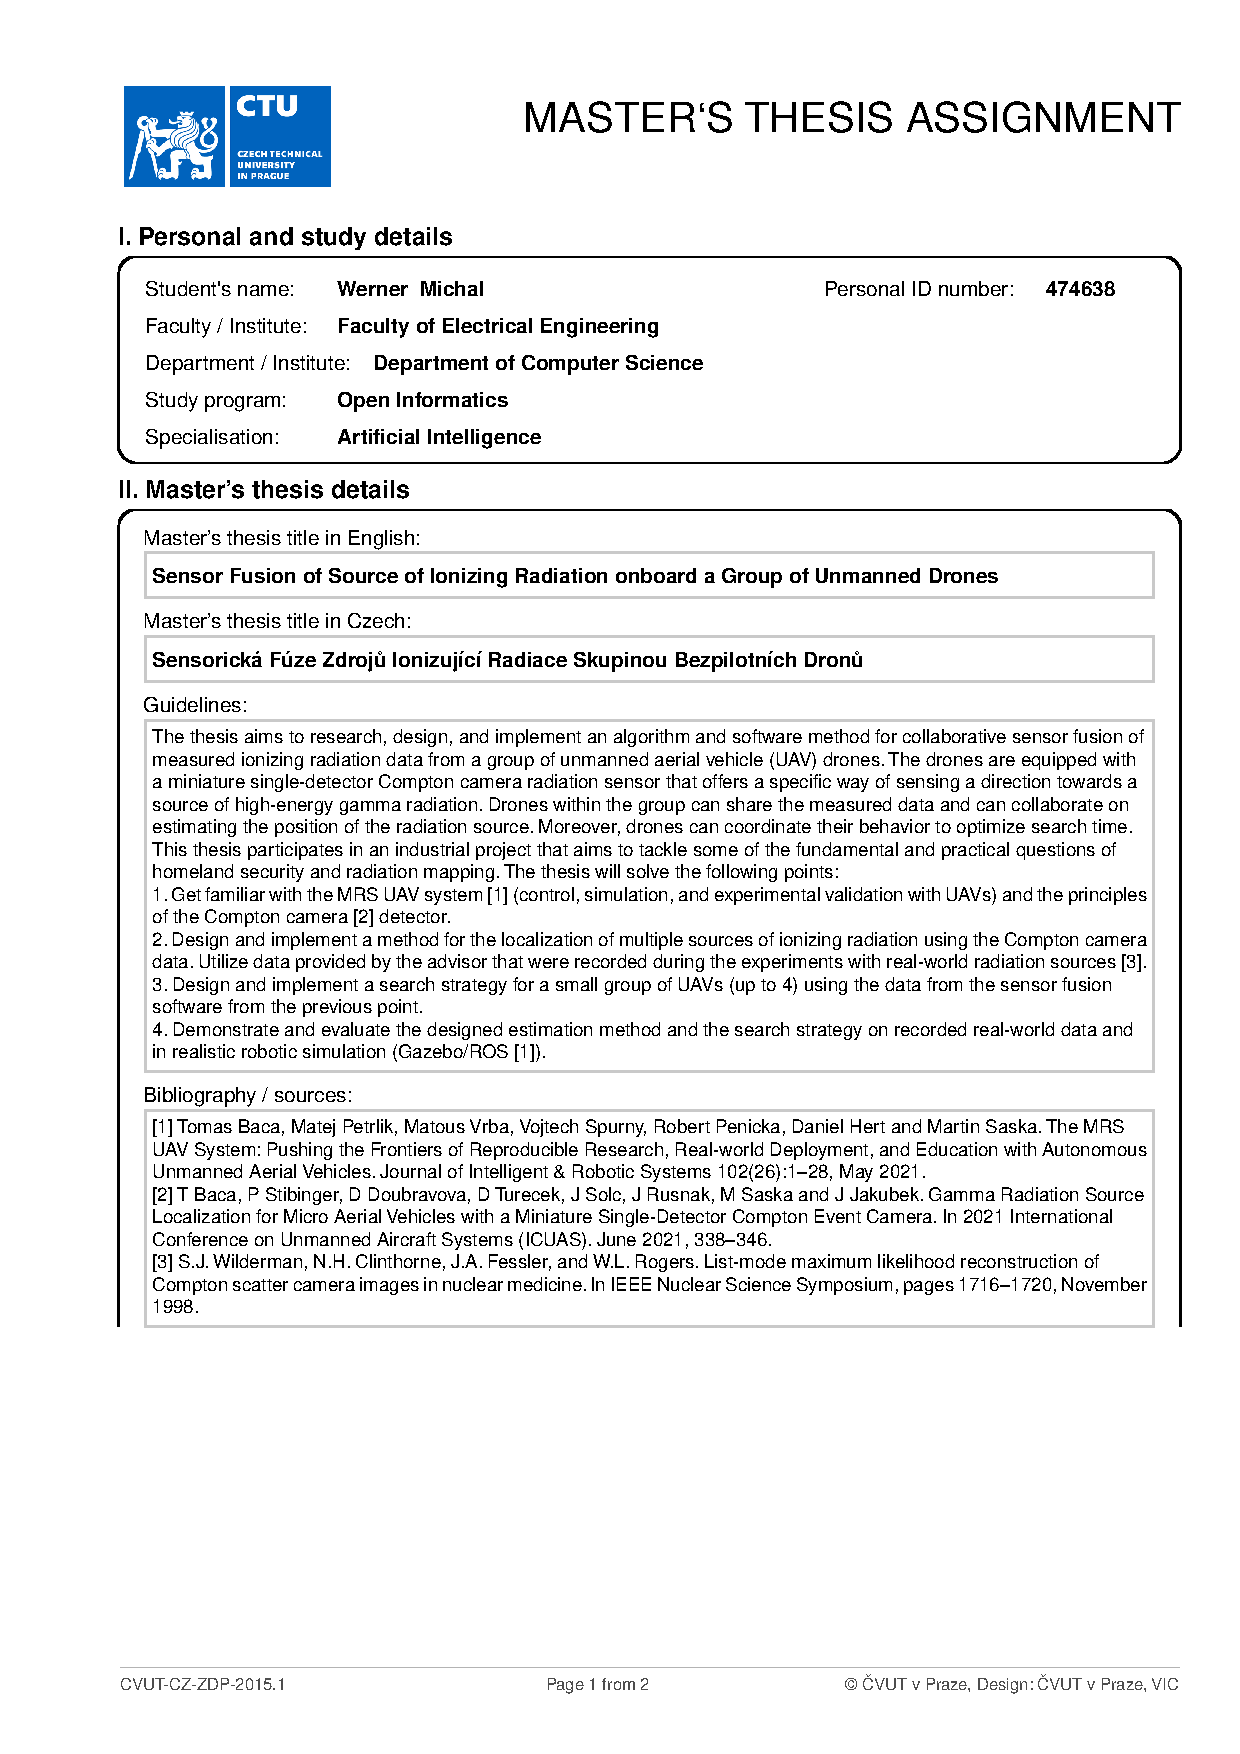
\includepdf{src/assignment.pdf}

%% --------------------------------------------------------------
%% |                          Abstracts                         |
%% --------------------------------------------------------------

\conditionalClearPage

%!TEX root = ../main.tex

\begin{changemargin}{0.8cm}{0.8cm}

~\vfill{}

\section*{Abstract}
\vskip 0.5em

This thesis presents a method for localizing multiple sources of ionizing radiation using a group of \acp{UAV}. 
These \acp{UAV} are equipped with miniature single-detector Compton camera radiation sensors, enabling them to estimate the directions towards high-energy gamma radiation sources.
  The proposed radiation mapping method (utilizing a \ac{MLE} principle) fuses the measurements from the Compton camera sensors to accurately estimate the positions of radioactive sources during the flight.
The properties of the used detector are approximated using Monte Carlo simulation techniques.
The estimation method is combined with an active search strategy that coordinates future action of the drones in order to improve the quality of estimate of sources position and minimize search time.
%In addition, an active search strategy is incorporated into the system, coordinating the future actions of the drones. 
%This strategy aims to improve the quality of the estimated source positions and minimize the search time by efficiently exploring the designated area of interest.
The proposed solution is evaluated on recorded real world data and in realistic simulator.





  \mycomment{
%The study of autonomous \acp{UAV} has become a prominent sub-field of mobile robotics.

This thesis presents a method for localization of multiple sources of ionizing radiation using a group of autonomous \acp{UAV} 
that are equipped with a miniature single-detector Compton camera radiation sensor capable of estimating directions towards a source of high-energy gamma radiation.
The proposed radiation mapping method (based on a \ac{MLE} principle) fuses the measurements from the Compton camera sensors and estimates the positions of radioactive sources during the flight.
Properties of the detector are approximated using Monte Carlo simulation.
The estimation method is combined with an active search strategy that coordinates future action of the drones in order to improve the quality of estimate of sources position and minimize search time.
The solution is evaluated on recorded real world data and in realistic simulator.
%The proposed estimation method based on maximum likelihood principle fuses the Compton camera measurements and estimates the positions of radioactive sources during the flight.
%The MiniPIX TPX3 Compton camera is can electronvolt
%The proposed solution utilizes a data fusion method based on \ac{MLEM} algorithm, which combines measurements from multiple \acp{UAV} and estimates the positions of radioactive sources during the flight.
%The fusion method 

%  for fusing the measurements
%and estimating the radiation source position during the flight.
}
\vskip 1em

{\bf Keywords} \Keywords

\vskip 2.5cm

\end{changemargin}


\conditionalClearPage

%!TEX root = ../main.tex

\begin{changemargin}{0.8cm}{0.8cm}

~\vfill{}

\section*{Abstrakt}
\vskip 0.5em

\sloppy
Výzkum na poli autonomních bezpilotních prostředků (UAV) se stal významným oborem mobilní robotiky.

\vskip 1em

{\bf Klíčová slova} \KlicovaSlova

\vskip 2.5cm

\end{changemargin}


%% --------------------------------------------------------------
%% |                        Abbreviations                       |
%% --------------------------------------------------------------

\conditionalClearPage

\begin{changemargin}{0.8cm}{0.8cm}

~\vfill{}

\section*{Abbreviations}

% this will print only the used abbreviations
%!TEX root = ../main.tex

\begin{acronym}
  \acro{API}[API]{Application Programming Interface}
  \acro{CTU}[CTU]{Czech Technical University}
  \acro{DOF}[DOF]{degree-of-freedom}
  \acro{FOV}[FOV]{Field of View}
  \acro{GNSS}[GNSS]{Global Navigation Satellite System}
  \acro{GPS}[GPS]{Global Positioning System}
  \acro{IMU}[IMU]{Inertial Measurement Unit}
  \acro{MLE}[MLE]{Maximum likelihood estimation}  
  \acro{LKF}[LKF]{Linear Kalman Filter}
  \acro{pix}[Minipix3]{MiniPIX TPX3}
  \acro{CS}[CS]{Compton scattering}
  \acro{PE}[PE]{Photoelectric effect}
  \acro{PET}[PET]{Positron emission tomography}
  \acro{SPECT}[SPECT]{Single Photon Emission Computed Tomography}
  \acro{FDNPP}[FDNPP]{Fukushima Daiichi Nuclear Power Plant}
  \acro{LM-MLEM}[LM-MLEM]{List-Mode Maximum Likelihood Expectation Maximization}
  \acro{MLEM}[MLEM]{Maximum Likelihood Expectation Maximization}
  \acro{MAP}[MAP]{Maximum A Posteriori}
  \acro{SOE}[SOE]{Stochastic Origin Ensemble}
  \acro{CC}[CC]{Compton camera}
  \acro{TSP}[TSP]{Travelling salesman problem}
  \acro{MAV}[MAV]{Micro Aerial Vehicle}
  \acro{MPC}[MPC]{Model Predictive Control}
  \acro{MRS}[MRS]{Multi-robot Systems Group}
  \acro{ROS}[ROS]{Robot Operating System}
  \acro{SLAM}[SLAM]{Simultaneous Localization And Mapping}
  \acro{UAV}[UAV]{Unmanned Aerial Vehicle}
  \acro{UGV}[UGV]{Unmanned Ground Vehicle}
\end{acronym}


\vskip 2.5cm

\end{changemargin}

\conditionalClearPage

%% --------------------------------------------------------------
%% |                      Table of contents                     |
%% --------------------------------------------------------------

\tableofcontents

\conditionalClearPage

% set up the full page style with normal page numbering
\pagestyle{full}
\pagenumbering{arabic}

%% --------------------------------------------------------------
%% |                        introduction                        |
%% --------------------------------------------------------------

%!TEX root = ../main.tex

\chapter{Introduction\label{chap:introduction}}

First, introduce the reader to the research topic.
Start with the most general view and slowly converge to the particular field, sub-field, and the challenges you face.
You can cite others' work here \cite{baca2021mrs}.

\section{Related works}

This section should contain related state-of-the-art works and their relation to the author's work.
We usually cite the original works like this \cite{benallegue2008high}.
You can also cite multiple papers at once like this \cite{baca2016embedded, baca2021mrs}.




\subsection{ MRS paper}
This thesis builds on the work of the MRS group (Faculty of Electrical engineering, CTU in Prague) in the field of radiation mapping. 
This paper \cite{baca2021gamma} presents a multi-robotic approach to an autonomous localisation of a compact gamma radiation source. 
All unmanned aerial vehicles are equipped with compact MiniPIX TPX3 CdTe event camera, which is capable of measuring gamma particles and reconstructing Compton events. 
The output of the sensor are Compton cones are used for localisation in the following way:
in the first phase of autonomous exploration, the \ac{UAV}s are exploring the area to measure the first Compton cones. 
After the first eight cones are reconstructed, their intersection is computed using optimisation methods (quadratic programming). 
This initial estimate is then incrementally updated using new measurements. 
The current estimate is always orthogonally projected to the newly measured cone. 
These measurements are fused using \ac{LKF}. 
The \ac{UAV}s are controlled in a way that they encircle the current estimate in order to measure more cones and update the \ac{LKF} estimate.

Using this approach, the group of drones is capable to localise a single compact source of ionising radiation. 
The source can be static or dynamic. 
However, this iterative method cannot localise multiple sources of radiation.
Once the drones detect one source of radioactive particles, they start encircling the current estimate and cannot find other sources in the area.

The main purpose of this thesis is to improve the presented solution: introduce a new method that could localise multiple sources of ionising radiation and control group of \ac{UAV}s to explore the whole area and maximise information gain given the specific sensor.



\section{TODO}
\begin{itemize}
\item clanek MRS ze ktereho vychazim
\item diplomka Petra Štibingera
\item ostatni robotické články týkající se robotickeho pruzkumu, leteckeho nebo pozemniho
\end{itemize}
\section{Contributions}

This section should describe the author's contributions to the field of research.

\section{Mathematical notation}

It is a good practice to define basic mathematical notation in the introduction.
See \reftab{tab:mathematical_notation} for an example.

\begin{table*}[!h]
  \scriptsize
  \centering
  \noindent\rule{\textwidth}{0.5pt}
  \begin{tabular}{lll}
    $\mathbf{x}$, $\bm{\alpha}$ & vector, pseudo-vector, or tuple\\
    $\mathbf{\hat{x}}$, $\bm{\hat{\omega}}$& unit vector or unit pseudo-vector\\
    $\mathbf{\hat{e}}_1, \mathbf{\hat{e}}_2, \mathbf{\hat{e}}_3$ & elements of the \emph{standard basis} \\
    $\mathbf{X}, \bm{\Omega}$ & matrix \\
    $\mathbf{I}$ & identity matrix \\
    $x = \mathbf{a}^\intercal\mathbf{b}$ & inner product of $\mathbf{a}$, $\mathbf{b}$ $\in \mathbb{R}^3$\\
    $\mathbf{x} = \mathbf{a}\times\mathbf{b}$ & cross product of $\mathbf{a}$, $\mathbf{b}$ $\in \mathbb{R}^3$\\
    $\mathbf{x} = \mathbf{a}\circ\mathbf{b}$ & element-wise product of $\mathbf{a}$, $\mathbf{b}$ $\in \mathbb{R}^3$ \\
    $\mathbf{x}_{(n)}$ = $\mathbf{x}^\intercal\mathbf{\hat{e}}_n$ & $\mathrm{n}^{\mathrm{th}}$ vector element (row), $\mathbf{x}, \mathbf{e} \in \mathbb{R}^3$\\
    $\mathbf{X}_{(a,b)}$ & matrix element, (row, column)\\
    $x_{d}$ & $x_d$ is \emph{desired}, a reference\\
    $\dot{x}, \ddot{x}, \dot{\ddot{x}}$, $\ddot{\ddot{x}}$ & ${1^{\mathrm{st}}}$, ${2^{\mathrm{nd}}}$, ${3^{\mathrm{rd}}}$, and ${4^{\mathrm{th}}}$ time derivative of $x$\\
    $x_{[n]}$ & $x$ at the sample $n$ \\
    $\mathbf{A}, \mathbf{B}, \mathbf{x}$ & LTI system matrix, input matrix and input vector\\
    \emph{SO(3)} & 3D special orthogonal group of rotations\\
    \emph{SE(3)} & \emph{SO(3)}~$\times~\mathbb{R}^3$, special Euclidean group\\
  \end{tabular}
  \noindent\rule{\textwidth}{0.5pt}
  \caption{Mathematical notation, nomenclature and notable symbols.}
  \label{tab:mathematical_notation}
\end{table*}


%% --------------------------------------------------------------
%% |                How to write thesis in LaTeX                |
%% --------------------------------------------------------------

%!TEX root = ../main.tex

\chapter{How to write thesis in LaTeX\label{chap:how_to}}

\section{Versioning with git}

Write the LaTeX in such a way that it could be versioned by git, which will help when collaborating with other people.
This means writing \textbf{one sentence per line}.
Even when you use third-party platforms, such as the OverLeaf, you can still share the repository through Git.

\section{Mathematical notation with LaTeX}

Use bold to visually distinguish vectors and matrices ($\mathbf{x}$, $\mathbf{A}$) and scalars ($k$, $N$).
Mathematical equations should be numbered and should be part of a sentence.
For example, the following equation is a discrete LTI system update
\begin{equation}
  \mathbf{x}_{\left[k+1\right]} = \mathbf{A}\mathbf{x}_k + \mathbf{B}\mathbf{u}_k,
  \label{eq:lti_system}
\end{equation}
where $\mathbf{x}_k \in \mathbb{R}^m$ is the state vector at the sample $k$, $\mathbf{u}_k \in \mathbb{R}^n$ is the input vector, $\mathbf{A} \in \mathbb{R}^{m \times m}$ is the main system matrix, and $\mathbf{B} \in \mathbb{R}^{m \times n}$ is the system input matrix.
Proper punctuation should be used after \refeq{eq:lti_system}, as if it were an ordinary object in the sentence.
Do not put any empty lines around the equation.
That would create a new paragraph mid-sentence.

\section{Using footnotes}

Do not be afraid to use footnotes for additional information, such as http links\footnote{This repository: \url{https://github.com/ctu-mrs/thesis_template}.}.
We use footnote links whenever we want to \emph{point} to a website, rather then to cite it as a source.
Like with everything, do not overdo it.

\section{Referencing to document elements}

LaTeX allows you to dynamically reference to parts of the documents, such as
\begin{itemize}
  \item figures: \reffig{fig:uavs}, Figure\,\ref{fig:uavs},
  \item equations: \refeq{eq:lti_system},
  \item code: \reflst{lst:references},
  \item and any other object that can contain \texttt{label}.
\end{itemize}

Check the section in the \texttt{document\_setup.tex} that contains useful macros for unifying the references:

\begin{lstlisting}[caption={LaTeX macros for referencing to document elements.},label={lst:references}]
  \newcommand{\reffig}[1]{Fig.~\ref{#1}}
  \newcommand{\reflst}[1]{Lst.~\ref{#1}}
  \newcommand{\refalg}[1]{Alg.~\ref{#1}}
  \newcommand{\refsec}[1]{Sec.~\ref{#1}}
  \newcommand{\reftab}[1]{Table~\ref{#1}}
  \newcommand{\refeq}[1]{\eqref{#1}}
\end{lstlisting}

\section{Abbreviations with Acronym}

Abbreviations are handled by the \emph{acronym} package.
Example sentence with abbreviations: ``\ac{UAV} is a flying vehicle that commonly uses \ac{LiDAR} and \ac{GPS} receiver''.
Please, read the documentation\footnote{Acronym package: \url{http://mirrors.ctan.org/macros/latex/contrib/acronym/acronym.pdf}}.

\section{Units of measurements with Siunitx}

Typesetting of units has never been more accessible with the Siunitx package.
Acceleration is measure in \si{\meter\per\second\squared}.
Gravity accelerates objects at a rate $\approx \SI{9.81}{\meter\per\second\squared}$ near the sea level.
You can define your units if you want.

Becquerel: $ \SI{10}{\mega\becquerel} $

\section{2D Diagrams with Tikz}

\emph{Tikz} is a powerful tool for drawing 2D (and 3D) shapes and diagrams.
Check the documentation and examples: \url{https://www.overleaf.com/learn/latex/TikZ_package}.
The benefit of using \emph{Tikz}, instead of some other third-party drawing program, are:
\begin{itemize}
  \item fonts are the same as in LaTeX,
  \item you can typeset math in LaTeX,
  \item you can use references to other parts of your document,
  \item you can version the image in git,
  \item the images are easily adjustable while editing your document.
\end{itemize}
Check \reffig{fig:pgfplots} for example.

\begin{figure}[!h]
  \centering

  \begin{adjustbox}{max totalsize={0.6\textwidth}{0.90\textheight}, center}
    \tikzset{
  >=stealth',
  punkt/.style={
    rectangle,
    rounded corners,
    draw=black, very thick,
    text width=5.7em,
    minimum height=2em,
    text centered,
  },
  small_punkt/.style={
    rectangle,
    rounded corners,
    draw=black, very thick,
    text width=4.0em,
    text centered,
  },
  arrow/.style={
    ->,
    very thick,
    shorten <=2pt,
    shorten >=2pt,
  },
  arrow_red/.style={
    ->,
    draw=red, very thick,
    shorten <=2pt,
    shorten >=2pt,
  },
}

\begin{tikzpicture}[node distance=1cm, auto,]

  % outer circle nodes
  \node[punkt] (sensor) {Sensor size};
  \node[punkt, inner sep=5pt, below = of sensor, shift = {(-6.0, -0.75)}] (aircraft) {Aircraft\\size};
  \node[punkt, inner sep=5pt, below = of sensor, shift = {(0.0, -4.0)}] (constraints) {Environment constraints};
  \node[punkt, inner sep=5pt, below = of sensor, shift = {(6.0, -0.75)}] (strategy) {Localization strategy};

  % inner circle nodes
  \node[small_punkt, inner sep=5pt, below = of sensor, shift = {(0.0, 0.5)}] (sensor2) {\scriptsize Sensor size};
  \node[small_punkt, inner sep=5pt, right = of aircraft, shift = {(0.5, -0.0)}] (aircraft2) {\scriptsize Aircraft\\size};
  \node[small_punkt, inner sep=5pt, above = of constraints, shift = {(0.0, -0.5)}] (constraints2) {\scriptsize Environment\\constraints};
  \node[small_punkt, inner sep=5pt, left = of strategy, shift = {(-0.5, -0.0)}] (strategy2) {\scriptsize Localization\\strategy};

  \path[->] ($(sensor.west)+(0, 0)$) edge [arrow,bend right=45] ($(aircraft.north)$);
  \path[->] ($(aircraft.south)+(0, 0)$) edge [arrow,bend right=45] ($(constraints.west)$);
  \path[->] ($(constraints.east)+(0, 0)$) edge [arrow,bend right=45] ($(strategy.south)$);
  \path[->] ($(strategy.north)+(0, 0)$) edge [arrow,bend right=45] ($(sensor.east)$);

  % inner circle paths
  \path[->] ($(sensor2.west)+(0, 0)$) edge [arrow_red, bend right=45, dashed] ($(aircraft2.north)+(0.0, 0.0)$);
  \path[->] ($(aircraft2.south)+(0, 0)$) edge [arrow_red, bend right=45, dashed] ($(constraints2.west)+(0.0, 0.0)$);
  \path[->] ($(constraints2.east)+(0, 0)$) edge [arrow_red, bend right=45, dashed] ($(strategy2.south)+(0.0, 0.0)$);
  \path[->] ($(strategy2.north)+(0, 0)$) edge [arrow_red, bend right=45, dashed] ($(sensor2.east)+(0.0, 0.0)$);

  % outer inner arrows
  \draw [->] ($(sensor.south)+(0, 0)$) -- ($(sensor2.north)$) node [midway, shift = {(0.0, 0.0em)}] {smaller};
  \draw [->] ($(aircraft.east)+(0, 0)$) -- ($(aircraft2.west)+(0.0, 0.0)$) node [midway, shift = {(0.0, 0.0em)}] {smaller};
  \draw [->] ($(constraints.north)+(0, 0)$) -- ($(constraints2.south)+(0.0, 0.0)$) node [midway, shift = {(0.0, 0.0em)}] {more complex};
  \draw [->] ($(strategy.west)+(0, 0)$) -- ($(strategy2.east)+(0.0, 0.0)$) node [midway, shift = {(0.0, 0.0em)}] {smarter};

\end{tikzpicture}

  \end{adjustbox}

  \caption{Example of a 2D diagram using tikz \emph{PGFPlots}.}
  \label{fig:pgfplots}
\end{figure}

\section{Data plots with PGFPlots}

\emph{PGFPlots} produces nice 2D and 3D data plots from data stored in CSV.
The plot parameters can be versioned and easily adjusted by editing the plot definition file.
\begin{itemize}
  \item Documentation and manual: \url{https://ctan.org/pkg/pgfplots}
  \item Compile the plots individually and then include the pdfs because it can take longer.
  \item Example located in \texttt{fig/plots/example\_plot}, see \reffig{fig:pgfplots}.
  \item You could include the latex file directly. However, it will take longer to compile, and platforms such as Overleaf can have a problem with that.
\end{itemize}

\begin{figure}[!h]
  \centering
  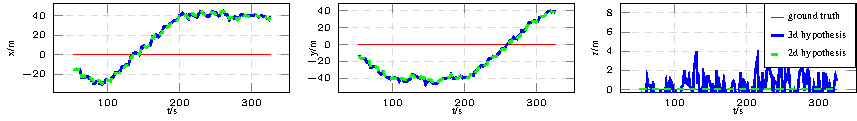
\includegraphics[width=1.0\textwidth]{./fig/plots/example_plot/hypotheses.pdf}
  \caption{Example of a 2D plot using \emph{PGFPlots}.}
  \label{fig:pgfplots}
\end{figure}

\section{3D Plots with Sketch}

\emph{Sketch} is a tool for defining a 3D scene using simple descriptive language.
The 3D scene is then converted to \emph{Tikz}, which is later compiled to pdf.
The benefits of using \emph{Sketch} are similar to using \emph{Tikz}: LaTeX fonts, versioning using git, and cleanness of the result.
See the example image in \reffig{fig:coordinate_systems}.
\begin{itemize}
  \item Documentation and manual: \url{http://www.frontiernet.net/~eugene.ressler/}
  \item Cross-compilation from \emph{Sketch} to \emph{pdf} using the \texttt{fig/sketch/compile\_sketch.sh} script.
\end{itemize}

\begin{figure}[!h]
  \centering
  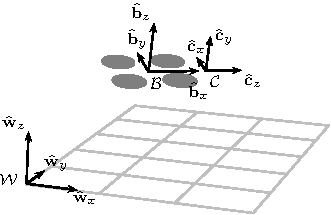
\includegraphics[width=0.4\textwidth]{./fig/sketch/coordinate_frames.pdf}
  \caption{Depiction of the used coordinate systems. The image was drawn using \emph{Sketch}.}
  \label{fig:coordinate_systems}
\end{figure}

\section{Image collages with Subfig}

We recommend using the \emph{subfig} packages, which provides the \emph{subfloat} command.
It is more versatile than the simpler \emph{subcaption} package.
Check the \reffig{fig:uavs} for example.

\begin{figure}[!h]
  \centering
  \subfloat[A UAV, the T650 model.] {
    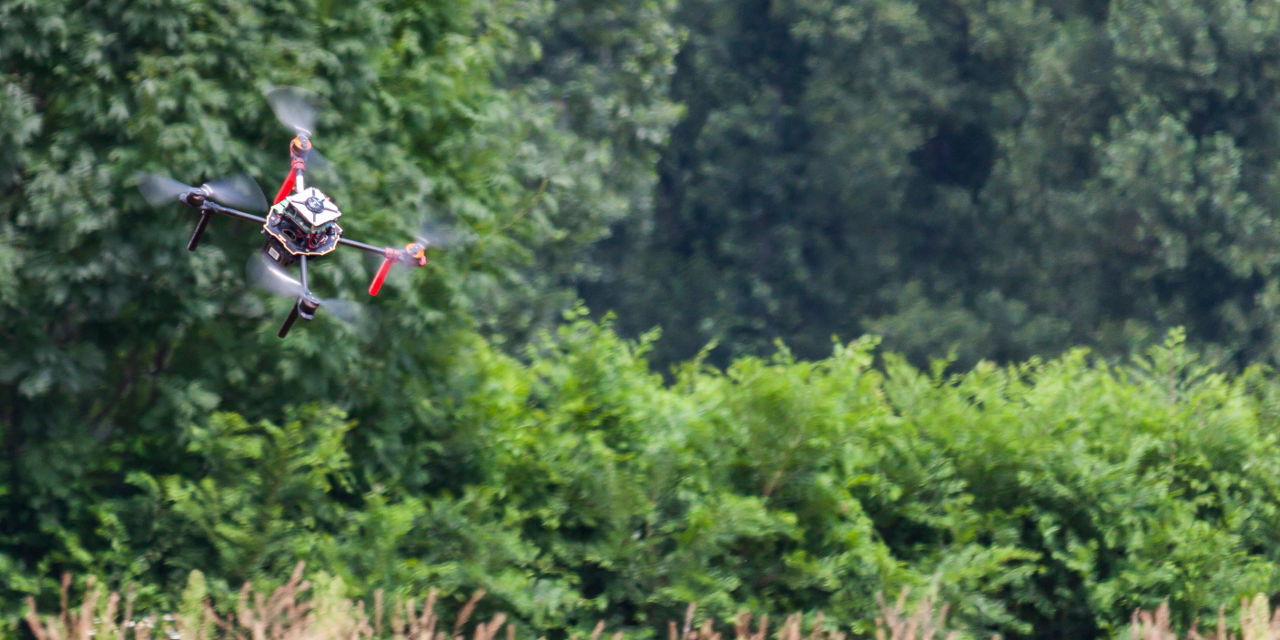
\includegraphics[width=0.48\textwidth]{./fig/photos/uav1.jpg}
    \label{fig:uavs_1}
  }
  \subfloat[Another UAV, again, T650 model.] {
    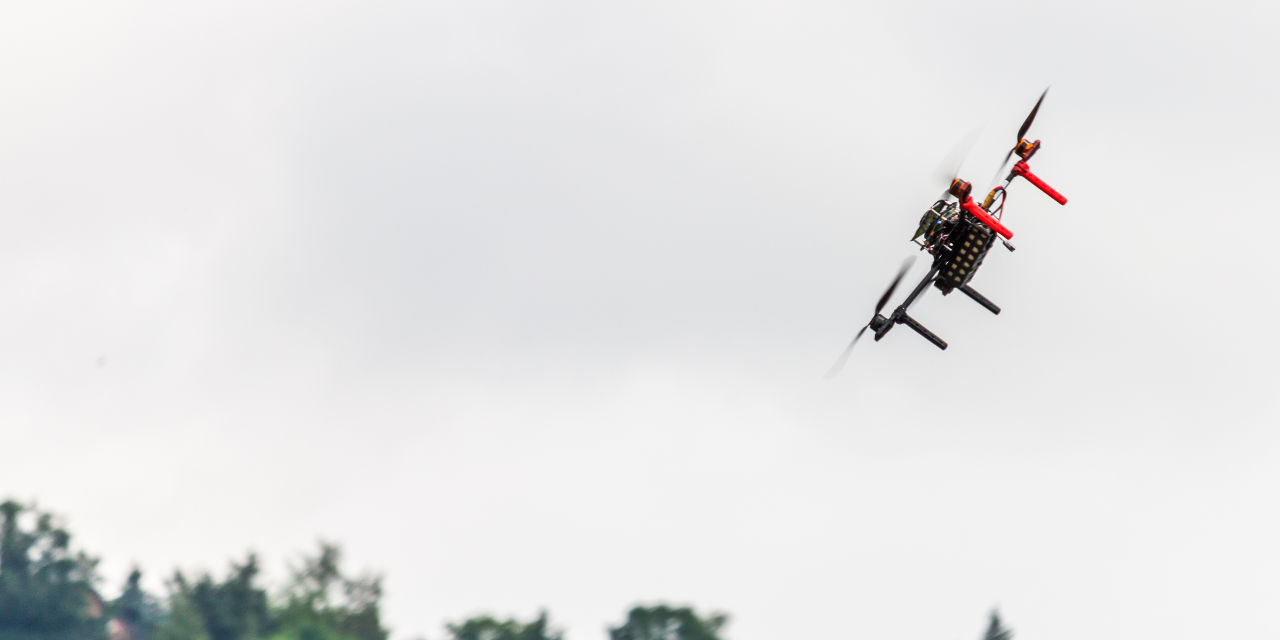
\includegraphics[width=0.48\textwidth]{./fig/photos/uav2.jpg}
    \label{fig:uavs_2}
  }
  \caption{The caption should mention both, the \reffig{fig:uavs_1} and the \reffig{fig:uavs_2}. You can just refer to them as (a) and (b), but beware, you need to keep it correct as you edit.}
  \label{fig:uavs}
\end{figure}

\section{Citations with Biblatex}

\emph{Biblatex} is probably the most powerful citation package for LaTeX.
It consumes the standard \texttt{.bib} file. However, it can sort and filter the citations using the \texttt{keywords} tag.
%Citing references is done using the \texttt{cite} command, e.g., \cite{baca2021mrs}.
You can also define some nice citation boxes, such as this one:
%\fullciteinbox{baca2021mrs}{}

\section{Image overlays with Tikz}

\emph{Tikz} is very useful to create custom image overlays.
The overlay can be set such that the image is spanned by Cartesian coordinates $\left(x, y\right) \in \left[0, 1\right]^2$
Example can be seen in \reffig{fig:tikz_overlay}.

\begin{figure}[!h]

  \centering

  \subfloat {\begin{tikzpicture}
    \node[anchor=south west,inner sep=0] (a) at (0,0) { 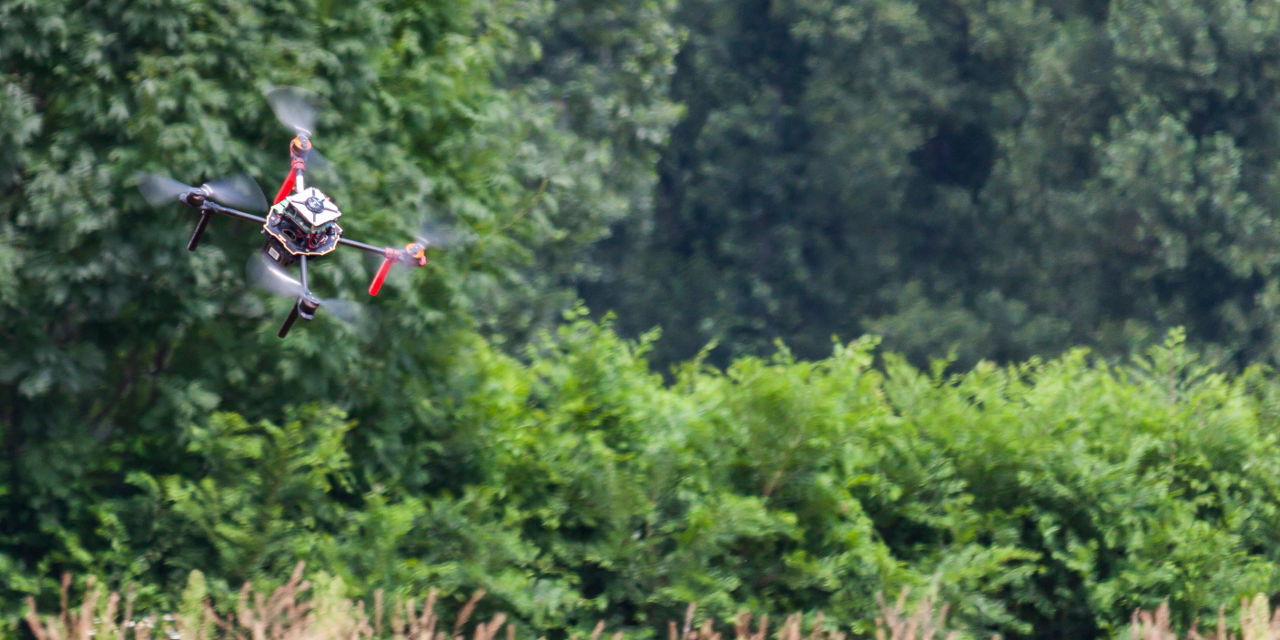
\includegraphics[width=0.45\textwidth]{./fig/photos/uav1.jpg}};
    \begin{scope}[x={(a.south east)},y={(a.north west)}]

      %%{ grid for placing the elements

      % % useful grid to help you find coordinates for plotting the overlay
      % \draw[black, xstep=.1, ystep=.1] (0,0) grid (1,1);
      % \foreach \i in {0,0.1,0.2,0.3,0.4,0.5,0.6,0.7,0.8,0.9,1} {
      %   \node[align=center] at (\i, -0.05) {\i};
      %   \node[align=center] at (\i, 1.05) {\i};
      %   \node[align=center] at (-0.05, \i) {\i};
      %   \node[align=center] at (1.05, \i) {\i};
      % }

      %%}

      % plot some stuff over the image

      % plot white background behind the letter (a)
      \fill[white] (0.001, 0.001) rectangle (0.08,0.14);

      % plot black border
      \fill[draw=black, draw opacity=0.5, fill opacity=0] (0,0) rectangle (1, 1);

      % write the letter (a) in the bottom-left corner
      \draw (0.04,0.06) node [text=black] {\small (a)};

      % plot black border
      \draw[->, white, thick] (0.50, 0.80) -- (0.30, 0.67);
      \draw (0.50,0.86) node [text=white] {\small \textbf{UAV}};
    \end{scope}
  \end{tikzpicture}}
\hfill%
\subfloat {\begin{tikzpicture}
    \node[anchor=south west,inner sep=0] (a) at (0,0) { 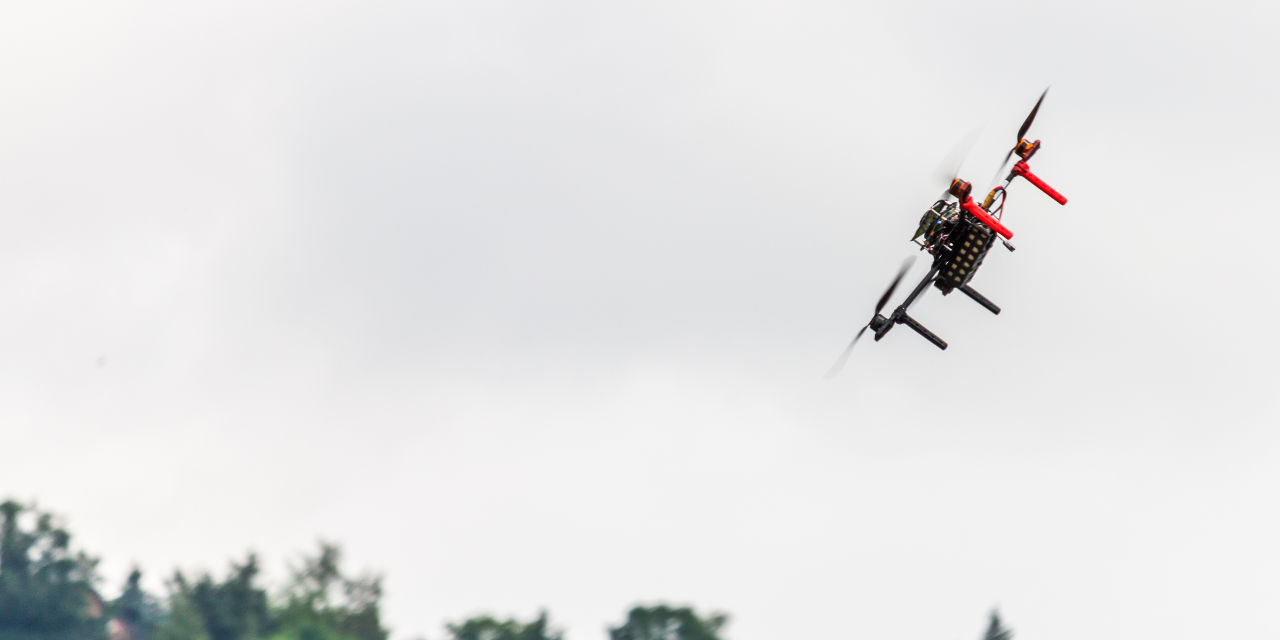
\includegraphics[width=0.45\textwidth]{./fig/photos/uav2.jpg}};
    \begin{scope}[x={(a.south east)},y={(a.north west)}]

      %%{ grid for placing the elements

      % useful grid to help you find coordinates for plotting the overlay
      \draw[black, xstep=.1, ystep=.1] (0,0) grid (1,1);
      \foreach \i in {0,0.1,0.2,0.3,0.4,0.5,0.6,0.7,0.8,0.9,1} {
        \node[align=center] at (\i, -0.05) {\i};
        \node[align=center] at (\i, 1.05) {\i};
        \node[align=center] at (-0.05, \i) {\i};
        \node[align=center] at (1.05, \i) {\i};
      }

      %%}

      % plot some stuff over the image

      % plot white background behind the letter (b)
      \fill[white] (0.001, 0.001) rectangle (0.08,0.14);

      % plot black border
      \fill[draw=black, draw opacity=0.5, fill opacity=0] (0,0) rectangle (1, 1);

      % write the letter (b) in the bottom-left corner
      \draw (0.04,0.06) node [text=black] {\small (b)};
    \end{scope}
  \end{tikzpicture}}


  \caption{Example of using Tikz for image overlays. (a) shows a final product, (b) shows a grid useful for nailing down the coordinates.}
  \label{fig:tikz_overlay}

\end{figure}


%% --------------------------------------------------------------
%% |                         Conclusion                         |
%% --------------------------------------------------------------

%!TEX root = ../main.tex

\chapter{Conclusion\label{chap:conclusion}}

Summarize the achieved results.
Can be similar as an abstract or an introduction, however, it should be written in past tense.


%% --------------------------------------------------------------
%% |                         References                         |
%% --------------------------------------------------------------

\chapter{References}

\printbibliography[heading=none,title={}]

%% --------------------------------------------------------------
%% |                         Appendices                         |
%% --------------------------------------------------------------

\appendix
\renewcommand\chaptername{Appendix}

\renewcommand{\thechapter}{A}
\renewcommand\chaptername{Appendix A}

\chapter{Appendix A}

\end{document}
